\chapter{Implementation}
\label{chap:implementation}

This chapter details the technical implementation of the TEKUTOKO platform, translating the architectural designs and requirements from the preceding chapters into a functional system. It covers the chosen technology stack, the development of the frontend and backend components with illustrative code snippets, the integration of external services, and the deployment strategy.

\section{Development Environment and Technology Stack}
\label{sec:impl-stack}
The technology stack was selected to optimize for developer productivity, performance, scalability, and a rich, modern user experience. The key technologies are summarized in Table \ref{tab:tech-stack}.

\begin{longtable}{p{3cm} p{3cm} p{8cm}}
\caption{Technology Stack and Rationale} \label{tab:tech-stack} \\
\toprule
\textbf{Component} & \textbf{Technology / Library} & \textbf{Rationale} \\
\midrule
\endfirsthead

\multicolumn{3}{l}{\tablename\ \thetable{}: Technology Stack and Rationale \textit{(continued)}} \\
\toprule
\textbf{Component} & \textbf{Technology / Library} & \textbf{Rationale} \\
\midrule
\endhead

\midrule
\multicolumn{3}{r}{\textit{(continued on next page)}} \\
\endfoot

\bottomrule
\endlastfoot

\textbf{Frontend} & \textbf{React 18 (with Vite)} &
A high-performance library for building dynamic, component-based SPAs.
Vite provides a significantly faster development experience than traditional bundlers. \\[0.5em]

\textbf{Styling} & \textbf{Tailwind CSS} &
A utility-first CSS framework that enables rapid, consistent, and responsive UI development directly within the JSX markup. \\[0.5em]

\textbf{Backend (Core)} & \textbf{Node.js / Express.js} &
A lightweight and efficient JavaScript runtime, ideal for building fast, scalable, and I/O-intensive REST APIs and handling real-time connections. \\[0.5em]

\textbf{Backend (Microservice)} & \textbf{Python 3 / FastAPI} &
A high-performance and robust framework for building the specialized DOCX parsing microservice, leveraging Python's strong ecosystem for data processing and managing external processes. \\[0.5em]

\textbf{Database} & \textbf{MySQL} &
A reliable, widely-used relational database system that ensures data integrity and supports complex queries required for analytics and user data management. \\[0.5em]

\textbf{File Storage} & \textbf{Firebase Storage} &
A scalable and secure cloud storage solution that simplifies file uploads and management through its powerful SDKs and direct-to-cloud upload capabilities. \\[0.5em]

\textbf{AI Service} & \textbf{Google Gemini API} &
A state-of-the-art large language model used for the AI Question Generator, capable of understanding complex prompts and producing high-quality, structured JSON output. \\[0.5em]

\textbf{Deployment} & \textbf{Vercel, Docker} &
Vercel provides seamless CI/CD and optimized hosting for the React frontend.
Docker is used to containerize the backend services for consistent, portable deployment. \\[0.5em]

\end{longtable}


\section{Frontend Implementation (React.js)}
\label{sec:impl-frontend}
The frontend is a Single-Page Application (SPA) structured to promote modularity and reusability. The codebase is organized by features (e.g., `components/room`, `components/test`, `pages/Discovery`).

\subsection{Anti-Cheating Logic in \texttt{TestRoom} Component}
A key implementation is the proctoring system within the `TestRoom` component. It uses React's `useEffect` hook to attach and clean up browser event listeners, ensuring monitoring only occurs during an active test session. The code is shown in Listing \ref{lst:proctoring-jsx}.
\FloatBarrier
\begin{lstlisting}[language=JSX, caption={Simplified anti-cheating logic in the `TestRoom` React component.}, label={lst:proctoring-jsx}]
import React, { useEffect, useState, useCallback } from 'react';
import { logProctorEvent } from '../../api/testService'; // API call

const TestRoom = ({ roomId, userId }) => {
  const [warnings, setWarnings] = useState(0);

  // Use useCallback to memoize the logging function
  const handleSuspiciousActivity = useCallback(async (eventType, details) => {
    console.warn(`Suspicious activity: ${eventType}`, details);
    setWarnings(prev => prev + 1);
    try {
      await logProctorEvent(roomId, userId, { eventType, details });
    } catch (error) {
      console.error("Failed to log proctoring event:", error);
    }
  }, [roomId, userId]);

  useEffect(() => {
    // Handler for tab/window visibility change
    const handleVisibilityChange = () => {
      if (document.hidden) {
        handleSuspiciousActivity('tab_switch', 'User switched tab.');
      }
    };

    // Handler to prevent and log paste attempts
    const handlePaste = (e) => {
      e.preventDefault();
      handleSuspiciousActivity('paste_attempt', 'User tried to paste.');
    };
    
    document.addEventListener('visibilitychange', handleVisibilityChange);
    document.addEventListener('paste', handlePaste);

    // Cleanup function to remove listeners when component unmounts
    return () => {
      document.removeEventListener('visibilitychange', handleVisibilityChange);
      document.removeEventListener('paste', handlePaste);
    };
  }, [handleSuspiciousActivity]);

  return (
    <div>
      {/* Test content goes here */}
      <div className="proctor-warning">Warnings: {warnings}</div>
    </div>
  );
};
\end{lstlisting}

\FloatBarrier
\subsection{GPS-Based Room Discovery}
The "Nearby" feature uses the browser's Geolocation API. Upon user consent, it retrieves the device's coordinates and sends them to the backend to find geographically close rooms.
\FloatBarrier
\begin{lstlisting}[language=JSX, caption={Logic for finding nearby rooms using the Geolocation API.}]
import React, { useState } from 'react';
import { findNearbyRooms } from '../../api/discoveryService';

const Discovery = () => {
  const [nearbyRooms, setNearbyRooms] = useState([]);
  const [isLoading, setIsLoading] = useState(false);

  const handleFindNearby = () => {
    if (!navigator.geolocation) {
      alert("Geolocation is not supported by your browser.");
      return;
    }
    
    setIsLoading(true);
    navigator.geolocation.getCurrentPosition(async (position) => {
      const { latitude, longitude } = position.coords;
      const rooms = await findNearbyRooms(latitude, longitude);
      setNearbyRooms(rooms);
      setIsLoading(false);
    }, () => {
      alert("Unable to retrieve your location.");
      setIsLoading(false);
    });
  };
  // ... JSX to render button and rooms
};
\end{lstlisting}
\FloatBarrier

\section{Backend Implementation (Node.js)}
\label{sec:impl-backend}
The Node.js backend uses Express.js to manage routing, middleware, and business logic.

\subsection{AI Question Generation with Prompt Engineering}
The `/api/rooms/generate-ai` endpoint demonstrates prompt engineering by constructing a detailed, structured prompt for the Google Gemini API. This ensures the model returns a predictable JSON object, simplifying parsing, as shown in Listing \ref{lst:prompt-engineering}.
\FloatBarrier
\begin{lstlisting}[language=JavaScript, caption={Backend service for generating questions via Gemini API with prompt engineering.}, label={lst:prompt-engineering}]
const { GoogleGenerativeAI } = require("@google/generative-ai");
const genAI = new GoogleGenerativeAI(process.env.GEMINI_API_KEY);

async function generateQuestions(topic, numQuestions) {
  const model = genAI.getGenerativeModel({ model: "gemini-pro" });

  const prompt = `
    You are an expert educational content creator.
    Generate a JSON object containing an array of ${numQuestions} questions 
    about "${topic}".
    Each question object must have: "question_text", "options" (an array
    of 4 strings), "correct_answer" (the correct string), and "explanation".
    Do not include any text or markdown formatting outside of the main JSON object.
  `;

  const result = await model.generateContent(prompt);
  const response = await result.response;
  const text = response.text();
  
  // Clean and parse the response to ensure it's valid JSON
  const jsonResponse = JSON.parse(text.replace(/```json/g, '').replace(/```/g, ''));
  return jsonResponse;
}

module.exports = { generateQuestions };
\end{lstlisting}
\FloatBarrier

\subsection{Secure Voucher Verification}
The `/api/vouchers/verify` endpoint handles QR code verification. It receives the unique data from the scanned code, queries the database to check its validity and redemption status, and performs an atomic update to prevent double-spending.

\FloatBarrier
\begin{lstlisting}[language=JavaScript, caption={Express.js route for secure voucher verification.}]
const express = require('express');
const router = express.Router();
const db = require('../config/db');
const authMiddleware = require('../middleware/auth');

router.post('/verify', authMiddleware, async (req, res) => {
  const { qrCodeData } = req.body;

  try {
    const [vouchers] = await db.promise().query(
      'SELECT * FROM vouchers WHERE qr_code_data = ?', [qrCodeData]
    );

    if (vouchers.length === 0) {
      return res.status(404).json({ error: 'Voucher not found.' });
    }
    const voucher = vouchers[0];
    if (voucher.is_redeemed) {
      return res.status(400).json({ error: 'Voucher already redeemed.' });
    }

    // Mark as redeemed
    await db.promise().query(
      'UPDATE vouchers SET is_redeemed = TRUE, redeemed_at = NOW() WHERE voucher_id = ?',
      [voucher.voucher_id]
    );
    res.status(200).json({ success: true, message: 'Voucher redeemed.' });
  } catch (error) {
    res.status(500).json({ error: 'Server error.' });
  }
});
\end{lstlisting}
\FloatBarrier

\section{Python Microservice for DOCX Processing}
\label{sec:impl-python}
The DOCX processing microservice is a critical component for handling user-generated content. It is a standalone Python application, containerized with Docker, that exposes a single API endpoint (`/api/v1/process-docx`) to perform a multi-step processing pipeline.

\subsection{The DOCX-to-JSON Pipeline}
The core logic of the microservice follows a strict sequence of operations to ensure reliable and consistent output. The entire flow is orchestrated by the `DocxService` class. The process is visualized in the flowchart below.

\begin{figure}[htbp]
\centering
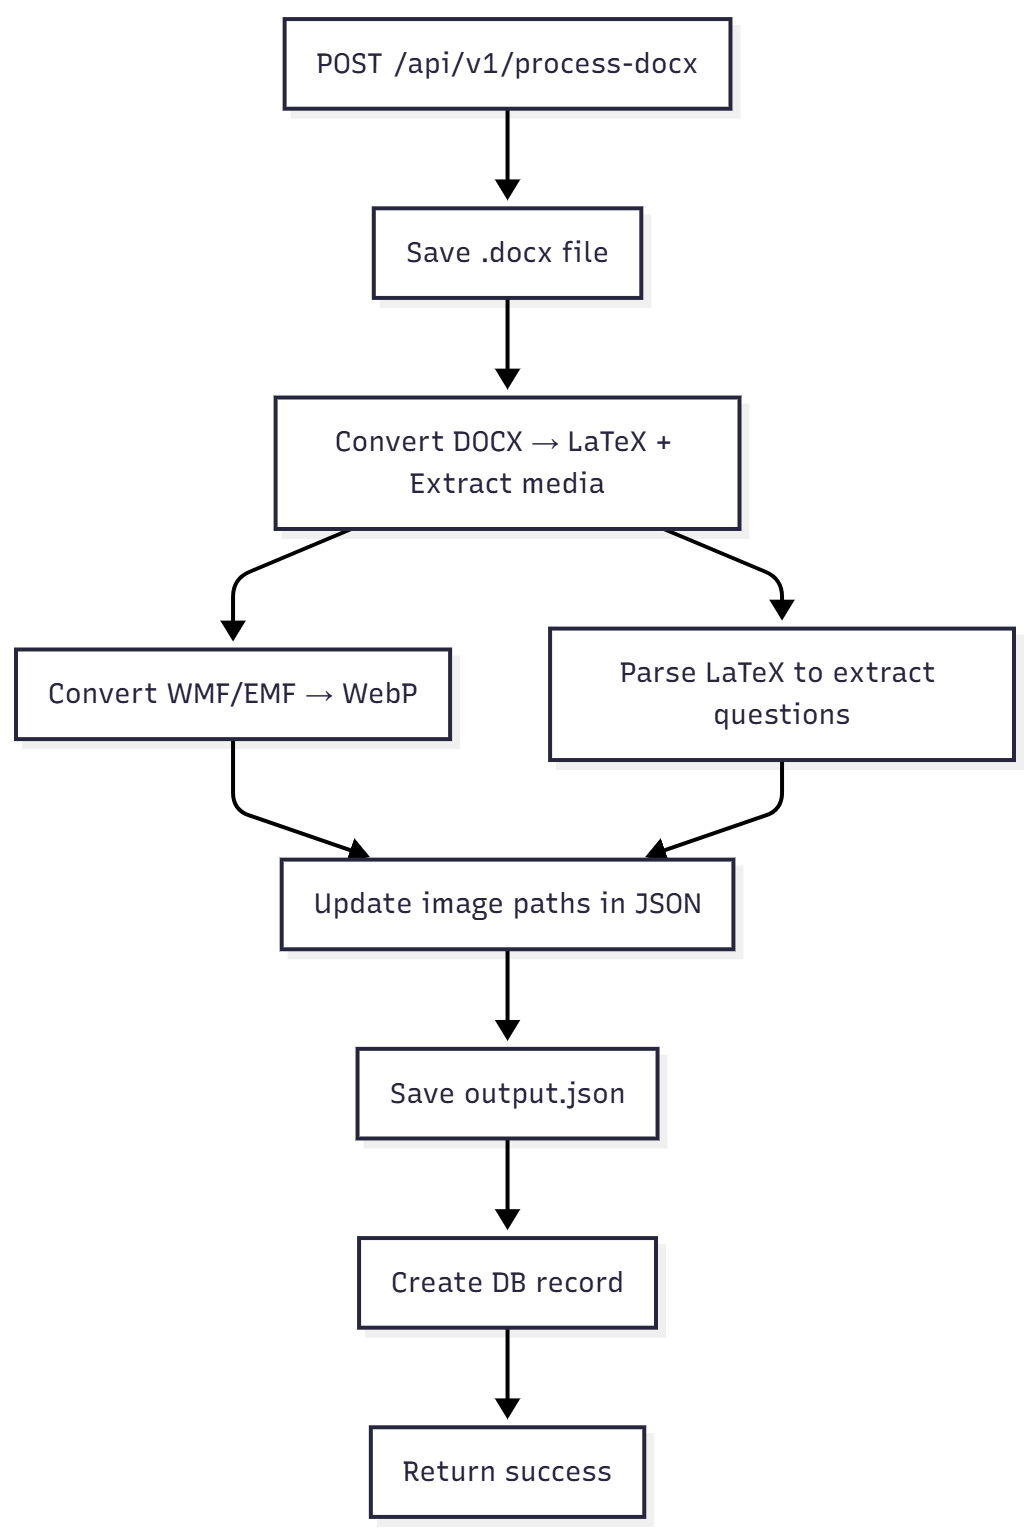
\includegraphics[width=0.9\textwidth]{figures/python-microservice-flow.png}
\caption{Flowchart of the DOCX Processing Pipeline}
\label{fig:python-microservice-flow}
\end{figure}

\FloatBarrier
\subsection{Orchestration and External Dependencies}
A key implementation detail is the interaction with external command-line tools. The service does not perform conversions natively but rather acts as an orchestrator.
\begin{itemize}
    \item \textbf{Pandoc:} Invoked via the `pypandoc` library to handle the initial conversion from DOCX to LaTeX. The `--extract-media` flag is crucial as it automatically saves all embedded images into a specified directory.
    \item \textbf{ImageMagick:} Called directly through Python's `subprocess` module. The `ImageUtils` class scans the extracted media directory for specific formats (like WMF, EMF) and uses a `ThreadPoolExecutor` to run multiple `magick convert` commands in parallel, significantly speeding up the processing of documents with many images.
\end{itemize}

The code in Listing \ref{lst:docx-service-py} illustrates how these steps are chained together within the main service class.

\FloatBarrier
\begin{lstlisting}[language=Python, caption={Illustrative logic of the `DocxService` in the Python microservice.}, label={lst:docx-service-py}]
import pypandoc
import os
from app.utils.image_utils import ImageUtils
from app.services.database_service import DatabaseService

class DocxService:
    def __init__(self, base_url: str):
        self.base_url = base_url

    def process_docx(self, input_path: str, uuid: str) -> dict:
        """
        Orchestrates the full DOCX processing pipeline.
        """
        output_dir = f"outputs/{uuid}"
        media_dir = os.path.join(output_dir, "media")
        
        # Step 1: Convert DOCX to LaTeX and extract media using Pandoc
        latex_output_path = os.path.join(output_dir, "output.tex")
        self.convert_docx_to_latex(input_path, latex_output_path, media_dir)
        
        # Step 2: Convert extracted images (WMF/EMF) to WebP using ImageMagick
        image_mapping = ImageUtils.convert_extracted_images(media_dir)
        
        # Step 3: Parse the intermediate LaTeX file to build a question structure
        questions_data = self.parse_latex_to_json(latex_output_path)
        
        # Step 4: Update image sources in the JSON with the final public URLs
        updated_questions = self.update_image_srcs(
            questions_data, uuid, image_mapping
        )
        
        # Step 5: Save the final JSON output
        final_json_path = os.path.join(output_dir, "output.json")
        self.save_output_json(updated_questions, final_json_path)

        # Step 6: Create an entry in the database
        DatabaseService.create_test_exam_room(uuid=uuid, title="Generated from DOCX")

        # Clean up temporary files like the .tex file
        os.remove(latex_output_path)
        
        return {"status": "success", "uuid": uuid}

    def convert_docx_to_latex(self, input_path, output_path, media_dir):
        # Wrapper for pypandoc call
        pypandoc.convert_file(
            input_path, 'latex',
            outputfile=output_path,
            extra_args=[f'--extract-media={media_dir}']
        )

    def parse_latex_to_json(self, latex_path):
        # Complex logic to parse LaTeX and extract question/option blocks
        # (Implementation omitted for brevity)
        pass

    def update_image_srcs(self, questions, uuid, mapping):
        # Logic to iterate through questions and replace local image paths
        # with final HTTP URLs using the self.base_url
        # (Implementation omitted for brevity)
        pass
    
    # ... other helper methods
\end{lstlisting}
\FloatBarrier

\section{Deployment and CI/CD Pipeline}
\label{sec:impl-deployment}
The deployment strategy is designed for automation, scalability, and separation of concerns.
\begin{enumerate}
    \item \textbf{Frontend (React):} The project is linked to a GitHub repository. A push to the `main` branch automatically triggers a new build and deployment on \textbf{Vercel}. Vercel's global CDN ensures fast load times for users worldwide. Environment variables for the backend API URL are managed through the Vercel dashboard.
    
    \item \textbf{Backend Services (Node.js \& Python):} Both the Node.js backend and the Python microservice are containerized using \textbf{Docker}. A `Dockerfile` in each service's directory defines its environment and dependencies. This includes installing system-level dependencies like `pandoc` and `imagemagick` for the Python service. These container images are pushed to a container registry (like Docker Hub or Google Container Registry) and can be deployed to any container orchestration platform like Google Cloud Run or AWS Fargate. This allows them to be scaled independently based on traffic and ensures a consistent runtime environment from development to production.
\end{enumerate}